%Old introduction

\section{Context}
In the study of cells, there are multiple methods which can be used to capture visual cellular data for observation and analysis. For the analysis of specific biological structures and molecules in visual isolation within specimens, the method known as fluorescent microscopy is of interest. This method uses wavelength-sensitive optical microscopes in combination with fluorescent indicators, also called fluorophores, which stain specific proteins which can compose organelles of interest.\citep{Sanderson-2014} For the study of mitophagy, the key organelles are the mitochondria, the subject of the mitophagy process, and both the autophagosomes and lysosomes. Throughout the mitophagy process, there are interactions between these three organelles biochemically and spatially which can be used to detect or observe mitophagy.
% Ask Rensu about the inclusion of Mitophagy here
\section{Problem Statement}
%Branches into organelles here by references to mitochondria and autophagosomes in prior section.
When imaging these organelles, or other similar structures, the capture of some quantity of noise within the image data is expected. The impact of this noise on the use of this data cannot be easily evaluated until after imaging through the use of other tools. A minor degree of noise is expected but as the presence of noise increases so do the challenges of working with the data for analysis. The difficulty of these aforementioned challenges is dependent on the severity of the noise and the sensitivity of the analysis method to be employed. Typically human evaluation, where a human visually evaluates the image data in terms of appearance, will be more robust to noise although less precise than a program which may use specific metrics which can be distorted by said noise even if imperceptible to the evaluating human. Due to this, it is important to apply a series of routines before analysing the image data to remove as much of this noise as possible without affecting the data of interest. Many of the steps of these routines can be automated or standard parameters can be used to reduce noise but one step used to isolate valid image data from the noisy data is thresholding. Correct use of thresholding is of great importance as the correct method must be used for the given data and depending on the method employed there is a risk of substantive amounts of noise being retained or valid data being removed. Many of these methods in the cellular physiology field require image analysis insight and understanding of the primary features of the employed method to correctly threshold the data and depending on the researcher these skills could be insufficient. 
%Could be better phrased as a section, especially in reference to noise and human evaluation
\section{Research Proposition}
The research proposition is to enable cellular physiologists, and potentially other disciplines, to benefit from a method that can automatically achieve thresholding with a sufficient quality outcome. The stipulation of "sufficient" here is important as there is currently no measure by which to determine the quality of a threshold save for comparison to a manually thresholded image but this manual thresholding will incorporate bias from the monitor used for the visual evaluation of the manual thresholding and the personal bias of the individual performing the thresholding towards the selected threshold values (i.e. an individual may feel it is better to err the threshold parameter higher or lower based on personal experience). The shortcoming of this is that there is a lack of consistency in this approach thus multiple experts can produce different thresholded images despite sharing an identical image prior to thresholding. This method will produce a consistent result (it shall always be the same for that exact image) and the quality will be sufficient such that incredibly experienced experts may prefer to perform their thresholding but for insufficiently skilled or experienced experts this method can produce results sufficient for further evaluation. The final aspect of this method is that it must process samples at a rate equal to or faster than an inexperienced researcher and that it must be capable of processing large quantities of data sequentially for efficiency.
\section{Research Question}
As this is a novel area of research the primary question is whether this method can be used to attain results of a consistent quality that is deemed sufficient for use by researchers. The method will currently expect the data to be either 2D or 3D and if a timelapse then the individual timeframes are to be individually thresholded. Prior steps in the preprocessing pipeline are of importance as the quality of the prior steps will determine the quality of the sample to be thresholded but these steps are not a focal point for evaluation thus all data used in evaluation will be prior to thresholding and all evaluations will be done relative to data sharing the same preprocessing pipeline. The thresholds will be determined for Hysteresis thresholding as it is easier to relate thresholds acquired from the proposed method to the low and high thresholds required for Hysteresis thresholding. Other techniques such as Adaptive thresholding, while performing well with manually determined parameters, can be challenging to relate to the histogram as the input parameters are not intensity-based which potentially eliminates the involvement of the image histogram in the parameter selection.
%This can be re-evaluated later with perhaps a second opinion. The content is currently more accurate but there is also a distinctive lack of references

\begin{figure}
    \centering
    \begin{subfigure}[t]{0.3\textwidth}
        \includegraphics[scale=0.7]{figs/widefieldApparatus.jpg}
        \caption{Wide-Field Microscope}
        \label{subfig:WFM}
    \end{subfigure}
    \hfill
    \begin{subfigure}[t]{0.69\textwidth}
        \includegraphics[scale=1.1]{figs/confocalApparatus.jpg}
        \caption{Confocal Microscope}
        \label{subfig:CM}
    \end{subfigure}
    \caption{Diagrams representing the Wide-Field Microscope and the Confocal Microscope \cite{Sanderson-2014}}
    \label{fig:microscope_diagrams}
\end{figure}

%**********************************************************************************************************

\section{Colocalisation quantification}
%Will need to rewrite for better wording and to adjust references to prior subsections. Have the listing of method names reference a paper that reviews or mentions all of these methods by some name which will be used for the subsection titles.
Depending on the research being performed, the analysis of the relationships and interactions between microscopic organisms and/or substances might be required. In the context of fluorescence microscopy the observation of these interactions are based on the relative positioning between different types of said organisms/substances where each type is labelled by a channel associated with the wavelength of the fluorescence. These fluorescence channels are discrete groups for the different fluorescence which have been captured and can be visually indicated using a distinct colour mapped to the respective channel. Where these colour overlaps can be perceived as a potential site of interaction between the structures that these respective colours represent and this method of analysis is referred to as colocalisation. For example, two types of organelles within a cell can be stained each with a different fluorophore and the interaction between these two organelle types can be evaluated visually where the mixture of the two colours will display the potential regions of interaction. colocalisation evaluation in a specimen can follow two distinct approaches with respective benefits and drawbacks which are visual and quantitative evaluation.\par The visual evaluation of colocalisation within an image, similar to the example described prior, where the observed regions of colour mixing (the overlap of fluorescence belonging to different channels) are termed as likely regions of colocalisation. After these likely regions have been identified, a human can employ their intuition and knowledge to determine the strength of the colocalisation. This visual evaluation is advantageous as it is easy to employ after imaging; a vast range of inconsistencies or aberrations in the image can be compensated for by the experience and/or knowledge of the human; and the granularity of the qualitative measurements for these regions can be adapted to the needs of the analysis. Despite these benefits the primary drawback of visual evaluation of colocalisation is due to the ambiguity of the results. The results of visual evaluation depend on distinctly interpreting the colour combination yet a clear combined colour relies on the intensities of each colour being similar \cite{practical_guide_coloc}. For example, if the colocalisation is being measured between two channels $R$ and $G$ where channel $R$ is presented as red and channel $G$ is presented as green. The visual colocalisation will be characterized by the overlap of the red and green colours which in digital colouring (\gls{rgb}) will appear as yellow. The prominence of yellow within an overlap region is reliant on the proportion of red and green within the region being similar. Due to the strength and confidence of the colocalisation within a region being estimated by the intensity of the colour yellow in the example above, visual colocalisation for a specimen is dependent on the fluorescence throughout the specimen being fixed and close in proportion \cite{practical_guide_coloc}. These drawbacks impact precise analysis of colocalisation of a sample but it can still function as an easily implemented estimate of colocalisation throughout the specimen.\par colocalisation quantification is a set of colocalisation methods that allow the occurrence and significance of the colocalisation throughout the specimen to be measured through image analysis. For this section the fluorescence colours which are emitted from distinct fluorophores binding to specific fluorophore will be categorized as colour channels. Measuring colocalisation between two channels within an image numerically allows certain relationships between the channels to be taken into account such as the relative proportion and distribution of the channel intensities throughout the image. Depending on the quantification method used, these relative intensities can be compensated for to accurately describe the colocalisation when the fluorescence being disproportional throughout the specimen or the positioning of this fluorescence between the channels. The methods which are often used are Pearson's coefficient, Mander's coefficient, Costes' approach, Van Steensel's approach and Li's approach \cite{Bolte-2006}. These methods though can only provide information regarding colocalisation across the entire specimen or within bounded regions of the specimen but they are unable to localize the proportion of colocalisation. When a measure of the colocalisation within a specimen and the spatial distribution of said colocalisation throughout the specimen is desired then a method called \gls{racc} \cite{racc}.
%Naming to be adjusted. Subsections must be a paragraph that is concise and covers the gist of the approach. i.e. approach requires ROI selection and measures the overlap within a vacuole of A relative to B but not B relative to A, so use in this scenario/describes this. Briefly state shortcoming such as PCC value of 0 or 1 is an understood descriptor but a value in between represents a vague notion.
%Reference Bolte in above text and how it discusses PCC, Manders, Costes', Van Steensel's and Li's. In the actual subsections briefly detail what it represents, its pros, its cons and preferably a secondary source besides Bolte + creator for these claims. e.g. how MOC is worse than PCC
\subsection{Pearson's approach}\label{sec:pcc}
%Reference the original and the use of it in Manders
Pearson's approach entails the use of \gls{pcc} with one of the earliest applications of this coefficient in fluorescence microscopy to measure colocalisation in "Measurement of co-localization of objects in dual-colour confocal images" \cite{Manders}. In Eq. \ref{eq:pcc} \cite[p. 376]{Manders}, the equation for \gls{pcc} is shown where $R$ and $G$ represent the red and green colour channel intensities respectively. The subscript $i$ denotes the specific image pixel intensity currently considered and subscript $aver$ denotes the average intensity for the associated channel. 
\begin{equation}\label{eq:pcc}
    r_p = \frac{\sum_i (R_i-R_{aver})\cdot (G_i-G_{aver})}{\sqrt{\sum_i (R_i-R_{aver})^2\cdot\sum_i(G_i-G_{aver})^2}}
\end{equation}
The value of the correlation coefficient $r_p$ can range from $-1$ to $1$ where a value of $1$ stands for complete positive correlation, $-1$ stands for negative correlation and $0$ stands for no correlation \cite{Bolte-2006}. This coefficient measures the pixel specific covariance between the two channels and the subtraction of the channel intensity means provides a resilience against channel noise \cite{practical_guide_coloc}. The \gls{pcc} is a reliable metric for extreme values that are close to $1$, $-1$ or $0$ where these values have understood implications yet intermediate values between these aforementioned values are challenging to interpret. It is only when measured in comparative studies where the \gls{pcc} for multiple specimen can be compared \cite{practical_guide_coloc}. \gls{pcc} is typically applied across the entire image but since the measure takes the correlation across the entire image thus the proportion of the colocalisation region sizes relative to the image size is proportional to the affect on the \gls{pcc} value \cite{practical_guide_coloc}. An example of this is say that in a two channel image there is a single small region possessing strong colocalisation measured as a \gls{pcc} value close to $1$ yet when the \gls{pcc} is calculated across the whole image then the low correlation of the two channels across the image outside of the aforementioned region will reduce the \gls{pcc} value thus it is beneficial to calculate the \gls{pcc} within select regions of the image to improve the accuracy of the measure.
\subsection{Manders' coefficient}\label{sec:mc}
Manders' coefficient is typically refers to \gls{mcc} but a precursor to this coefficient is the \gls{moc} \cite{practical_guide_coloc}. The \gls{moc} is based off of \gls{pcc}, described in Section \ref{sec:pcc}, where the subtraction of the channel average is removed from the equation (seen in Eq. \ref{eq:pcc}) resulting in a coefficient that ranges from $0$ to $1$ in value providing, specifically, a measure of the overlap between the channels \cite{Manders} with a value that may be easier to interpret if the negative \gls{pcc} values caused confusion \cite{practical_guide_coloc}. This measure is functionally independent of the fluorescence proportionality within the image but is rather sensitive to co-occurrence (any level of overlap between) the channels thus the method is overly sensitive to the presence of noise and offsets in the channel can greatly impact the result. The second metric, \gls{mcc}, is technically composed of two measure $M_1$ and $M_2$ where each measure relates to the sum of the channel intensities across all pixels where the other channel intensity is non-zero and is divided by the sum of the intensities across the channel \cite{Manders}. The calculation for $M_1$, where $M_1$ represents the red channel, can be seen in Eq. \ref{eq:mcc} and to calculate $M_2$ the same equation will be used save that $R$ and $G$ will be swapped in the equation where $G$ represents the green channel in this description \cite{practical_guide_coloc, Manders}. Each $M$ coefficient (where the subscript denotes the focal channel specific measurement) are measures of the ratio of the proportion of channel intensity of the focal channel that overlaps with the other channel with respect to the total intensity of the focal channel. This ratio concerns the intensity of only a single channel signal with the only influence of the other channel being the spatial bounding of what pixel intensities can be evaluated in the numerator thus these measures can apply even when the channel intensities differ greatly from each other \cite{Manders}. These measures are still hampered by the presence background fluorescence (typically noise of some nature) which can lead to false positives for fluorescence coincidence thus \gls{mcc} has a sensitivity to noise. In summary \gls{mcc} is a more reliable \gls{moc} but it inherits the noise sensitivity of \gls{moc} requiring accurate preprocessing.
\begin{equation}\label{eq:mcc}
    M_1 = \frac{\sum_i R_{i,colocal}}{\sum_i R_i} \text{ where }
    \begin{cases}
    R_{i,colocal}=R_i,& \text{if } G_i>0\\
    R_{i,colocal}=0,& \text{if } G_i=0
    \end{cases}
\end{equation}
\subsection{Costes' colocalisation threshold method}
Costes' approach is an algorithm that aims to remedy the shortcomings of \gls{mcc} regarding the noise removal through the use of \gls{pcc} \cite{costes}. This algorithm is actually focused on the determination of a channel specific threshold for each evaluated channel to maximise the effectiveness of \gls{mcc}. This process entails two steps with the first evaluating the legitimacy of the \gls{pcc} measurement for the image and the second step shifting the channels thresholds with the \gls{pcc} value used as the selection criteria for said thresholds.\par For the first step the \gls{pcc} value is calculated between the two channels which will be the observed \gls{pcc} value $r_{obs}$ after which one channel will be selected as the scrambled channel. The scrambled channel will have its pixels (or blocks of pixels) randomly re-positioned within the channel image and the scrambled \gls{pcc} value will be measured. After $N$ repetitions of this scrambling process have occurred a probability density function relative to the \gls{pcc} can be constructed where the probability value (P-value) can be determined as the integral of the probability density function across all \gls{pcc} values with an upper bound of $R_{obs}$ \cite{Bolte-2006}. In the development of this algorithm by Costes' et al. \cite{costes}, the P-value cutoff was chosen to be $95\%$ to be deemed valid and the scrambled channel was scrambled 200 times. This P-value criteria was developed to aide in the reliability of the uncertain intermediate \gls{pcc} values by use of a statistical significance test \cite{costes}. This test utilized the scrambled channel to determine if the observed correlation was more reliable than the correlation results from random overlaps between the channels (the scrambled channel) \cite{costes}. If the P-value was too low then it meant that $r_{obs}$ was similar no more reliable than the \gls{pcc} value derived from a scrambled channel.\par If the first step is passed successfully then the second step is performed where the actual thresholds are acquired. For this method a linear relationship between the two channel intensities (and the potential threshold values) and the threshold is initially set high. With the threshold set the \gls{pcc} is calculated and after each calculation the thresholds are successively decremented until a \gls{pcc} of 0 is acquired \cite{practical_guide_coloc, costes}. The threshold values at the point where the \gls{pcc} is zero will be used as the thresholds for \gls{mcc}. This threshold mitigates the "noise" which can disrupt the reliability of the \gls{mcc} measures although there are conditions where it performs poorly such as images with low signal intensities (distance between background noise and true fluorescence is small) a threshold that is too low might be selected \cite{practical_guide_coloc}. The performance of the initial step is also dependent on the scramble repetitions used where the performance is improved with more repetitions \cite{Bolte-2006} although this does not affect the accuracy of the second step. This method performs best when applied to an image with sparse colocalisation pixels compared to images with high colocalisation pixel densities within the image \cite{costes}.
\subsection{Van Steensel's colocalisation}
Van Steensel's approach entails the calculation of \gls{pcc} between two channels and then one of the channels is shifted relative to the other channel image and the \gls{pcc} is calculated again for each shift \cite{vanSteensel}. In the paper this approach originated from (Van Steensel et al. \cite{vanSteensel}) the channels were chosen to be red and green and the shift was relative to the x-axis which is represented by $\delta x$ and a distribution of the \gls{pcc} value relative to the $\delta x$ was constructed and was called the \gls{ccf} \cite[p.223-225]{Bolte-2006}. This distribution would take the shape of a bell curve ideally and in the case of completely colocalised structures presented by a peak in the \gls{ccf} at $\delta x=0$. A difference in fluorescence intensity between the colocalised structures can manifest as wider peak or lower height, partial colocalisation manifests as a shifted peak which is not centred at $\delta x=0$. In cases of zero colocalisation the \gls{ccf} peak is a dip instead centred at, or near, $\delta x=0$ which means that there is no significant colocalisation. Colocalisation due to random overlap or high noise will manifest as a \gls{ccf} that is relatively flat \cite{Bolte-2006, vanSteensel}. The accuracy of this approach is heavily influenced by the shape and distribution of fluorescence throughout a continual structure relative to the axis shift \cite{Bolte-2006}. This limitation implies that applying this approach to structures with a high variance in the intensity spatially such that a shift $\delta x=-n$ and $\delta x=n$ will result in vastly different \gls{pcc} values relative to an isolated structure although the \gls{pcc} values when shifted in the y-axis do not have to be similar to the x-axis results, as mentioned they only need to be "symmetrical" along the shifted axis. Bolte et al. stated "...it is only valuable for small and isotropic particles, ..." \cite[p.225]{Bolte-2006}.
\subsection{Li's colocalization metrics}
Li's approach \cite{Li4070} was developed to determine if two proteins that were stained were part of the same protein complex (or structure) or if they belonged to other structures. This method was developed for the use case of detecting the presence of a biological relationship between two proteins but it can also be applied when determining if two bio-molecular components constitute a shared structure or complex. This method functions under the assumption that if two proteins (or components) are part of the same complex (or structure) then the variation in their staining intensity should be synchronised and if they are not synchronised then they are not part of the same complex \cite{Li4070}. Li et al. \cite{Li4070} referred to these dependent and segregated staining for stains on the same structure or on different structures respectively. The method of evaluating the type of staining occurring within a sample employs either the \gls{ica} or the \gls{icq} method where the \gls{icq} provides a singular value assessing the result of \gls{ica} \cite[p. 4079]{Li4070}. The \gls{ica} method is based on the principle that the sum of deviations from the mean equal zero (example in Eq. \ref{eq:sum_dev}) where  $a_i$ represents the intensity at pixel $i$ for channel $A$, which contains $N$ pixels, and $\overline{a}$ represents the intensity average across channel $A$ \cite[p. 4073]{Li4070}.
\begin{equation} \label{eq:sum_dev}
    \sum_N (a_i -\overline{a}) = 0
\end{equation}
The application of these principle in detecting the staining association between channel $A$ and channel $B$ assumed that the sum of products between each channels pixel intensity deviation from their channel mean would tend to zero as in Eq. \ref{eq:sum_dev} did not consistently hold. This was not an inherent issue though for the method this deviation from this assumption is what enabled the measurement of the relationship between the inter-channel staining dependency or segregation. The equation used to evaluate this relationship is shown in Eq. \ref{eq:ica} where the sign of the sum of products determine the type of staining across the evaluated region (which can be chosen to be the full image or a select region) \cite[p. 4073]{Li4070}. Using Eq. \ref{eq:ica}, normalised channel intensity scatterplots can be generated which are typically channel $A$ by channel $B$, channel $A$ by $(A-\overline{a})(B-\overline{b})$ and $B$ by $(A-\overline{a})(B-\overline{b})$ where $A$ and $B$ imply $a_i$ or $b_i$ for some pixel $i$ in the region. The scatterplots are not expected to be identical between each channel since the \gls{ica} value from Eq. \ref{eq:ica} is unchanged for both channel $A$ and $B$ but the distribution of the respective channel intensities relative to the \gls{ica} value are not identical. From these scatteplots it can be determined at what intensity ranges for a channel does that channel staining become dependent or segragated \cite{Li4070}.\par
\begin{equation}\label{eq:ica}
    \sum_N (a_i - \overline{a})(b_i - \overline{b}) \text{ where}
    \begin{cases}
    > 0 \text{ is dependent}\\
    < 0 \text{ is segregated}
    \end{cases}
\end{equation}
The second method of evaluation is more commonly used as it provides a single value thus accurate interpretation of a scatterplot in \gls{ica} is not required and a simpler representation of the staining relationship between channels can be determined. This value is measured as the ratio between the number of positive products of channel deviations from channel mean, $(A-\overline{a})(B-\overline{b}) > 0$, divided by the total number of products that would be summed which will be the number of pixels in the measured region $N$. This ratio is then subtracted by $0.5$ so that the range of results will be $-0.5<ICQ<0.5$ where, in Li et al. \cite[p. 4074]{Li4070}, $ICQ \approx 0$ describes random staining; $0<ICQ\geq 0.5$ implies dependent staining, and $-0.5\geq ICQ < 0$ implies segregated staining. Bolte et al. \cite[p. 227]{Bolte-2006} describe the relations of the \gls{icq} values regarding the staining relationship such that a value of $0.5$ represents colocalisation and $-0.5$ represents exclusion. \gls{ica} presents an improvement over visual evaluation of colocalization via the scatterplots as the properties described by the \gls{ica} scatterplots allow the staining relationship between the channels across the intensity ranges to be examined e.g. a large degree of segregated staining occurs at lower channel intensities while at high intensities there is dependent staining and for ideal specimen the determination of the staining relationship can be performed with further information available. \gls{icq} allows the inter-channel relationship to be 
numerically approximated in an easily interpreted manner although intermediate values can be challenging to accurately evaluate in a non-comparative study since the metric is only concerned with the ratio of positive pixel intensity deviation products between channels but not the measure of this product thus the intensity related information is reduced to provide this singular value metric \cite{Bolte-2006}.

\subsection{\gls{racc}}
\gls{racc} is a method, developed by Rensu et al. \cite{racc}, to both calculate colocalisation within a sample and to visualise the colocalisation within the sample spatially for a researchers interpretation. There exist many colocalisation metrics but they frequently struggle with the visualisation of colocalisation as they were not designed with that objective in mind and thus can struggle with spatially distributing the colocalisation metric value across the sample image \cite[p. 4]{racc}. \gls{racc} addresses this by achieving three primary aims such that it can be used as a reliable metric of colocalisation which is visualised by avoiding the limitations of visualising other colocalisation metrics. The first aim is the focus on colocalisation with a positive correlation while reducing the presence of negatively correlated and random colocalisation in the evaluated region. The second aim is to place significance on the combined channel fluorescence within colocalised regions such that larger combined fluorescence is emphasized. The third aim is the reduction of false positive colocalisations induced by coincidental or random colocalisations. Figure \ref{fig:racc_example} has been edited to place emphasis on the visualisation provided by \gls{racc} for only the "partially overlapping spheres" example from the original figure particularly visualises the "Overlap", "Colocalization", "RACC" and "Scatter plot" for this example. The views provided are from a 3D perspective and a 2D \gls{mipdef} perspective. From the aforementioned figure it can be seen that \gls{racc} provides a visualisation of purely the colocalized segment since only overlapping regions where both channel intensities are above a specific threshold are calculated for \gls{racc} and the intensity of the \gls{racc} visualisation in Fig. \ref{fig:racc_example} (displayed as magenta with varying brightness across the range) is dependent on the strength of the correlation at each point in the overlapping region \cite[p. 13-14]{racc}.

\begin{figure}
    \centering
    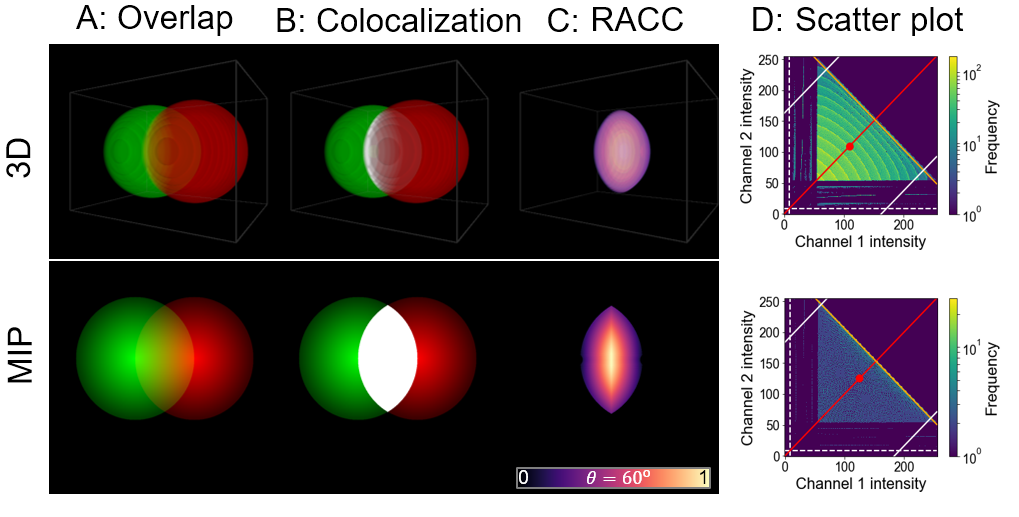
\includegraphics[width=\textwidth]{figs/raccSynth.png}
    \caption{Visualisation of overlap, colocalization and \gls{racc} with the associated scatterplot adapted from Rensu et al. \cite[p. 13]{racc}.}
    \label{fig:racc_example}
\end{figure}

%Mitophagy and mitochondria detail

\section{Mitochondria and Mitophagy}\label{sec:mito_detail}
%The core points of this section are mentioning mitochondria network morphology and the mitophagy process. These are the things seen in my data and are the feature being modeled
This section will provide a conceptual understanding of the mitochondria and their functions which define their importance within cells. There will be a focus, particularly on the purpose and process of mitophagy as that is the mentioned research of context (Section \ref{sec:prob_state}) that this system is to improve. For this reason, the biological information, microscopy techniques and algorithms discussed in this chapter are those that are either applied or explored in the context of mitophagy research. For this reason, not every potential option is explored here but rather the subset that played a role in the development journey of the system presented by this thesis to address the research question proposed in Section \ref{sec:res_que}.
\subsection{Mitochondrial Structure, Functions and Networks}
%This discusses the mitochondrial networks, a brief overview of their events and their purpose
\subsubsection{Mitochondrial Structure}
%Mention biomolecules from intro to physiology. It refers to biochemical units such as lipids, proteins and other molecules prevalent in the biological processes and functionality of the cell such as enzymes
%Consider figures involving mitochondria shape and a network structure
Mitochondria are rod-shaped organelles, subcellular structures with specific functions, found only in eukaryotic cells, cells with a nucleus encapsulated by a membrane. The mitochondrial structure is roughly rod-shaped and consists of two membranes, one enveloping the other, and the inner membrane has numerous inward folds. The surface of this inner membrane contains proteins and the internal cavity is filled with a fluid called the matrix which contains enzymes and DNA which are used in its range of functions.\cite{introPhys-2013}
\subsubsection{Mitochondria Functions} %Ca regulation is quite important in specific cell groups (perhaps mention the other functions they are involved in but do not detail) This could be summarised as well. All of the mitochondria functions are not of importance to me but just mention them and that ATP is king.
The mitochondria can perform a range of functions based on which cell type the organelle is situated in such that mitochondria in muscular cells might perform functions that are not performed by mitochondria in nerve cells. The most prominent function of all mitochondria irrespective of the host cell is the synthesis of ATP from food. Energy extraction is performed via a process called cellular respiration where oxygen and water is utilised in the mitochondria to extract energy from food molecules and to store it as Adenosine Triphosphate (ATP). This is important since the desired energy from digested food is typically trapped in a carbon-bond which the other organelles cannot access and despite the process of glycolysis being an option, the extract of ATP in the intracellular fluid through the use of enzymes, it is inefficient manner of ATP production which is insufficient for most eukaryotic cell processes in the long term. When the energy is extracted from ATP a phosphate is ejected and it becomes Adenosine Diphosphate which can return to the mitochondria for recharging. This recharging process allows multiple early steps to be skipped since most of the molecule is already present and this allows a method to significantly the rate at which the mitochondria supplies energy to the cell.\cite{introPhys-2013} \newline\newline Other important cell functions are the regulation of calcium within a cell which is utilized for signaling between cells for coordinated actions such as muscular contractions [source this]. Another key function is the management of Apoptosis. Apoptosis is the process in which the cell self-terminates based on certain signals and conditions. This typically occurs when the cell is no longer necessary or is dysfunctional. This essentially allows for the regulation of cell proliferation which can prevent scenarios such as tumor growth.[Verify if this is still a valid cite]\cite{Apopt-2009} While apoptosis is the intentional or programmed death triggered by the cell, there is another form of prevalent cell death called necrosis. Necrosis is the death and rupturing of cells in the body due to extreme cellular stress, or trauma, and can prove toxic to the surrounding cellular environment. While necrosis entails the swelling and rupturing of damaged cells, apoptosis is characterised as a shrinking of a cell where apoptosis is an energy demanding process. Cells that cannot produce sufficient ATP and do not correctly trigger apoptosis can proceed to necrosis which is undesirable.\cite{introPhys-2013}  
\subsubsection{Mitochondrial Networks and Behaviors} \label{sec:MitoNet}
%This can remain the same size but make sure that stress is a key player. These networks can be branched structures
Multicellular eukaryotic organisms differ from single celled organisms in the range of functions and actions they can perform through which they can adapt and endure a great variation of environmental conditions. A drawback of this variability is that these organisms require more energy depending on their complexity, the more cells that compose an organisms means that more energy is required. The supply of this energy at the required scale for these organisms would not be possible without mitochondria which are specialised for efficient energy extraction and storage but each mitochondria can only synthesise a certain amount of ATP at any given time. The result of this is that cells containing more mitochondria can facilitate more intensive functions and processes thus it is common for mitochondria to number from hundreds to thousands in the cells of multicellular organisms.\cite{introPhys-2013} This multitude of mitochondria have been observed to interact with each other within cells in order to perform a range of functions known as fusion and fission. These fission and fusion events have been noted to be a key player in maintaining sufficient ATP synthesis within the cell which is required for continued survival. Since this process relies on a collective of mitochondria it is the health of that collective which exceeds any individual mitochondria.\newline\newline The factors of interest that disrupt the ATP synthesis can be viewed as stresses. These stresses in the mitochondria context can be externally induced by environmental factors including heat, radiation and toxicity or internal factors such as mutations and reactive oxygen species (ROS) production. Of the internal factors listed the production of ROS is of great interest due to it being exclusive to mitochondria. ROS is a highly reactive anion which is a byproduct of ATP synthesis and it damages proteins, lipids and the mtDNA of the mitochondria which is of concern as those are components used for ATP synthesis. As this ROS induced damage accumulates within a mitochondria the ATP synthesis efficiency declines while ROS production further elevates. This damage is controlled and mitigated within the mitochondria through the use of enzymes which dispose of the damaged components while DNA repair processes are used to recover mtDNA damage. This is not infallible though as this relies on the damage afflicted by the ROS to be dealt with at a rate matching or exceeding the ROS production but this is not always definite and becomes less likely if further factors stress the mitochondria. Through ROS and other factors it is also not uncommon for mutations within the mtDNA to appear during repeated proliferation and an accumulation of these mutations can further stress the ROS damage mitigation systems. \newline\newline Here lies the purpose of the fusion and fission events across the mitochondrial collective. Fusion is a process where mitochondria connect and share components and mtDNA. This sharing of components allows healthy mitochondria to support damaged mitochondria by compensating for the damaged components and improving the ATP synthesis of that fusion. The sharing of mtDNA allows for complementation which means that mtDNA between mitochondria with different mutations can compensate for each other as long as a mutation threshold is not exceeded.\cite{MitoFus-2012} This fusion behaviour can lead to long, tubular mitochondrial networks forming to improve robustness and durability of the whole network as they support each other.\newline\newline Fission is the event where the mitochondrial damage cannot be managed within the organelle nor by fusion between mitochondria. The process is the same as binary fission which is the means through which mitochondria proliferate within a cell but here it is used for damage control. Fission is employed within networks in order to separate mitochondria and mitochondrial network segments that are beyond repair. For network separation it can be summarised as a cleaving of the membranes conjoined at the point of connection while within an individual mitochondria it is the division of the organelle into daughter organelles. This binary fission application differs to normal that the damaged material is segregated from the healthy material and are separated. This binary fission of damaged from healthy material culminates in a damaged daughter to be disposed of and an undamaged daughter to continue performing ATP synthesis.\cite{MitoFus-2012}
\subsubsection{Summary of these points}
%Might need some references for the punctuate and to reinforce the correlation between large degrees of fragmentation and stress
The primary functions of mitochondria across all bodily cells are the synthesis of ATP to meet energy needs and the management of Apoptosis so that damaged and unnecessary cells can be removed from the body without harm to surrounding cells. These demands on the mitochondria results in a large number of mitochondria being required both to meet the necessary rate of ATP replenishment and as backups for each other if some mitochondria become dysfunctional. The dysfunction of mitochondria can be attributed to either cellular stress or to the ROS produced during the process of ATP synthesis which accumulate and cause damage within the mitochondria. This ROS damage is mitigated to an extent by the organelle but to improve survivability and robustness in face of this growing damage and rising energy requirements mitochondria fuse with each other. These fusions can culminate in large networks which compensate for the individual organelles and can be potentially viewed as signs of mild but tolerable stress in the case of high increases of energy demand in active muscular cells. Another key event is the fission which is involved in mitochondria replication but also in isolating overly damaged mitochondria segments. These segments break away from the networks to be disposed of and can lead to many smaller structures to be present in the cytosol. In situations where the networks are closer to scattered particles (punctuate) than tubular networks then it can be a sign of extreme stress within the cell. The shape of these structures, or their morphology, across the mitochondria can be precursors to future cell behaviour and of current cell conditions.    
%Haven't mentioned network fragments or shapes in general (what about puncta?) This might need to be it's own subsection with subsubsections but Rensu can be queried on this. 
%Network fragmentation being an underlying indicator of stress but also disease is key: https://journals.plos.org/plosone/article?id=10.1371/journal.pone.0223014
\subsection{Mitophagy purpose and process}\label{sec:Mitophage}
%The conditions under which mitophagy usually occurs, how mitophagy happens (process), why it is important. Also mention mitochondrial biosynthesis crosstalk with mitophagy
Mitophagy can be characterised as autophagy performed on mitochondria where autophagy is the process used to break down organelles within a cell.\cite{introPhys-2013}  
\subsubsection{Mitophagy purpose}
%This can be reduced in size, make a summarised duplicate of the report and compare them afterwards
The purpose of mitophagy is the disposal of dysfunctional mitochondria which cannot be repaired. This is important as damaged mitochondria are not merely insufficient ATP suppliers but can also actively damage the function of the cell. Two of the possible consequences of these dysfunctional mitochondria, depending on the extent and location of the damage, are the consumption of ATP within the cell, which places further strain on the ATP synthesis capacity of the healthy mitochondria, and the unintentional triggering of apoptosis via the release of Cytochrome c. The consumption of ATP by damaged mitochondria is done to maintain the internal membrane potential of the mitochondria and this potential is disrupted by limited cellular respiration or leaks in the inner membrane.\cite{ATPconsum-2010} A membrane potential is the electrical potential across a membrane based on the distribution of electrons. This difference in charge, or potential, creates a gradient which facilitates the movement of molecules across the membrane based on their charge. In mitochondria there is a large collection of positively charged hydrogen molecules in the intermembrane space and they are placed there through the membrane potential during a phase of cellular respiration called Oxidative Phosphorylation. These hydrogens typically flow back into the inner membrane space via specific channels which drive the largest contributor to ATP synthesis in the process.\cite{introPhys-2013} If the inner membrane began leaking or was compromised that positive hydrogen could freely migrate back into the matrix then the driving force of the via the specific channels become minimal and the matrix needs to use energy to actively pump the hydrogen back into the intermembrane space. These pumping requires energy to be performed which is then sourced from ATP in the cytosol. ROF damage is primary cause of this damage as there are a range of oxidative and other stresses which contribute to cause this potential loss in the membrane.\cite{ATPconsum-2010} In energy demanding cells this ATP consumption can be disastrous and a primary cause of cell death due to energy starvation leading to necrosis.
\subsubsection{Mitophagy process}
%First paragraph regarding how damaged mitochondria or fragments are flagged, second paragraph introduces autophagosome as a structure and it's role in encapsulating/capturing mitochondria. Last paragraph is regarding the transportation to the Lyosome and briefly touch on the disposal but this is not a focal point as it would never be visible in my data
The process of mitophagy can be as a three stage process within a cell. These stages are the detection, capturing and decomposition of damaged mitochondria. Mitophagy can be selective or non-selective depending on the state of the mitochondria population within a cell and their condition. Non-selective mitophagy typically occurs in order to regulate healthy mitochondria populations through mitochondrial removal and decomposition. Selective mitophagy is induced for the removal of damaged mitochondria within a cell and specific biochemical markers are used to guide this process.\newline\newline In terms of selective mitophagy in mammalian cells, such as human cells, enzymes in the cytosol called Parkin bind to the damaged mitochondria acting as an identifier. These enzymes do not simply bind to any membrane surface or else there would be risk of incorrect flagging of organelles for autophagy. For mitochondria, Parkin binds with a protein called PINK1 which has been found to be within the intermembrane space and the inside of the outer membrane but it is not certain. Irrespective of the source of PINK1, PINK1 crosses into the inner membrane of the mitochondria where it is rapidly degraded by protealysis, the degradation of proteins by a protein-degrading enzyme. This happens shortly after the synthesis of PINK1 in healthy mitochondria thus PINK1 populations are typically quite low but in the event of sufficient mitochondrial damage the protealysis is inhibited. This allows the PINK1 count to grow and travel to the outer membrane where it is stable and can form protein complexes, protein based structures formed from groups of proteins binding together. Parkin proceeds to connect to the complex and act as a flag.\newline\newline With the damaged mitochondria being flagged a double-membrane structure called an autophagosome traverses through the cytosol and detects the flagged mitochondria and approaches it. Once the flagged mitochondria is within reach of the autophagosome, the autophagosome begins the process of enveloping the mitochondria. With this the mitochondria is isolated from the other organelles and can be transported by the autophagosome. With the mitochondria being transported the final stage of decomposition occurs. This stage entails the fusion of the autophagosome with organelles called lysosomes. After fusing an autolysosome is formed which has the capacity to degrade and break down the mitochondria into it's constituent components for reuse in the cell. The final two stages from mitochondria envelopment to the autolysosome formation are common to the base autophagic process within the cell for all organelles.\cite{MitoMechan}      

% old chapter 1

\section{Context}\label{sec:Context}
In the study of cells and their related phenomena, there is a myriad of analysis techniques that can be applied depending on the biological subjects being studied and the experiments being performed. Amongst these analysis techniques is the use of microscopy to visually image biological structures, chemicals and organisms to track changes and interactions between and within them. This evaluation can be performed by either a human through visual inspection or the application of image-based algorithms to determine metrics essential to the analysis. Due to this, it is crucial that the contents of the image are an accurate representation of the imaged specimen to provide credibility to the analysis results. This requirement of representation accuracy engenders the minimal presence of image noise, or other visual aberrations, that are detrimental to the accuracy. When these visual detriments, referring collectively to the aforementioned noise, are present it is essential that methods to erase said detriments be applied whilst preserving the actual representation.

\section{Problem statement}\label{sec:prob_state}
An analysis of the occurrence of a biological process called mitophagy is to be measured in specimens through visual evaluation for some given research. This mitophagy process involves multiple biological structures but the primary subjects of interest are the cellular organelles called mitochondria, autophagosomes and lysosomes. The process of mitophagy (detailed in Section \ref{sec:mito_detail}) is undergone when the autophagosomes and lysosomes interact with the mitochondria thus precise differentiation between these organelles and the visual isolation of these organelles from the remaining biological components within the cell is crucial. To further improve the accuracy of the observation of the organelle interactions further spatial resolution is desired. The details of the imaging technique applied to meet these demands are discussed in Section \ref{sec:fluorMicr} and the reasoning for the use of this technique is covered in Section \ref{sec:Dataset_making}.\par Irrespective of the technique applied, the removal of visual detriments from the image is essential in order to perform accurate evaluations by either people or, more so, by algorithms. This removal of image noise can be performed through a number of techniques applied individually or in concert (also detailed in Section \ref{sec:Dataset_making}) the threshold techniques enable the complete removal of undesired image elements. These threshold techniques decrease in intuitiveness relative to the complexity and frequency of these visual detriments such that human-involved threshold applications entail potentially time-expensive processes and accuracy dependent on the human applying said technique.

\section{Research proposition}
The proposition of this research is to target the threshold technique stage of the image-cleaning pipeline, where cleaning refers to the removal of visual detriments in the image, as the effective application of threshold techniques involving minimal human intervention increases in difficulty depending on the nature of these images. This automated system would provide consistent threshold results with minimal human bias and can be applied to large batches of samples. The performance of the system is expected to produce results of usable quality while being performed faster than an inexperienced human researcher could provide said results. The aim of the system is not to exceed the accuracy of researchers experienced in threshold applications but rather to provide a high throughput alternative to save time for large image volumes. Ideally, this will save experienced researchers time and aid researchers inexperienced in this threshold application by saving time and providing usable results thus removing a potential workflow bottleneck.

\section{Research question}\label{sec:res_que}
The research question proposed is whether a deterministic system is capable of producing threshold results that are sufficiently accurate for further and produced fast enough using purely characteristics derived from the sample image. To add further specificity, the system is expected to execute a result from a sample within the range of a minute; to remove visual detriments while favouring the preservation of the subjects of interest; and to perform for both 2D and 3D images.


%The below has been rewritten

\subsection{Solutions to restore image quality}
%For all of these methods at least one or two methods of interest can be directly named especially if there is not a "grouping" for techniques such as denoising techniques being sub-categorized as statistical or linear
To address these degradations in image quality there are multiple methods that have been developed which can be allocated to three groups. 
\begin{itemize}
    \item \textbf{Histogram-based methods}: make adjustments to the image using calculations employing the image histogram
    \item \textbf{Edge-based methods}: employ a number of techniques which are designed to retain different types of edges depending on the employed methods
    \item \textbf{Image-based methods}: these methods are based on pixel/voxel values across the whole image or for segments of varying sizes.
\end{itemize}
These groups are not rigid nor official but merely group these methods in regards to either a shared behaviour in terms of their process e.g the reliance on the image histogram or the intended outcomes of the method e.g. the detection and localization of edges within the image.
\subsubsection{Histogram-based methods}
%Need to discuss Gaussian Blurring, Speckle noise removal and filtering techniques. Try not to be overly specific else going to need to list many pointless methods that won't be used
Histogram-based methods are algorithms that employ the use of the image histogram to determine the changes to be made to the image. In terms of filters and thresholds the histogram is used to infer a desirable threshold value to be used to filter the image and remove undesirable elements. These methods are frequently designed to be automatic with merely a few input arguments which can be used to tune the results. Some of these methods are the Mean, Minimum, Yen, Triangle and Otsu thresholding. 
\subsubsection{Edge-based methods}
% This will be for the deconvolution methods such as Richard-Lucy and so forth. The list can be obtained from Deconvolution Lab2 with the methods briefly described. Pros and Cons do not need to be listed unless such specificity can be acquired from literature for most of the methods.
Edge-based methods utilize a range of algorithms to isolate edges within an image. What pixels/voxels get removed and what "type" of edges focused on depends on the algorithm employed. Some such methods are the Roberts Cross operator, the Sobel filter, the Scharr transform, the Farid transform, the Laplace operator and the Prewitt transform. Edge-based methods utilize edge detection to isolate perceived borders between shapes and objects through localized variations in intensities throughout an image. Edge detection methods reduce the total quantity of information within an image down to the edges of shapes and structures which can aid the use of image segmentation or recognition techniques. A shortcoming of many edge detection techniques is that they do not mitigate or effectively remove noise outside of the object edges.
\subsubsection{Image-based methods}
%This will be for filtering methods. Adaptive and Hysteresis are the most important to mention but Otsu, Triangle, Mean, Li, Yen and Mean can also be mentioned. Just describe the limitations of the method and the main caveats (Hysteresis can look for connected edges, adaptive also looks for connected edges but is better at separating structures)
Image-based methods are a set of methods that either employ algorithms to apply global changes across the image such as adjusting contrast or brightness throughout, these are not effective methods in removing noise but they can be used to support other methods to more effectively improve image quality. A few examples of these techniques are  \par Other image-based methods are those that adjust the image through algorithms that examine neighbourhoods of pixels/voxels, even if these neighbourhoods are the size of the complete image. Neighbourhoods are localized regions of pixels covering and area, or in the case of voxels a volume, and calculations are applied taking these localized collections into account. Similar approaches are used in many edge-based methods but these are performed without the inherent goal of isolating image edges. Of these methods two of particular interest are Hysteresis Thresholding\cite{Hysteresis} and Adaptive Thresholding. 

